%\documentclass[10pt,spanish,a4paper,openany,notitlepage]{article}
\documentclass[a4paper,10pt]{article}

%-------------------------------------Paquetes-----------------------------------------------------------------------
\usepackage[spanish]{babel}  	% Traduce los textos a castellano
\usepackage[utf8]{inputenc}	% Permite escribir directamente áéíóúñ
\usepackage{t1enc}            	% Agrega caracteres extendidos al font
\usepackage{amsmath} 		%Permite imprimir mas opcciones matematicas
\usepackage{graphicx}		%Permite agregar imagenes al informe
\usepackage{multicol}  		%Permite dividir el texto en varias columnas
\usepackage{anysize}		%Permite modificar los margenes del documento
\usepackage{float} 		%Permite utilizar H para colocar las imagenes en un lugar especifico 
\usepackage{units}

% Paquete para dividir las tablas en subtablas
\usepackage{multirow}

%estos 2 sirven para achicar la tabla
\usepackage{booktabs}
\usepackage{tabulary}

\usepackage[spanish]{babel}
%------------------------------------------------------------------------------------------------------------------------

%---------------------------------------Configuraciones de pagina-------------------------------------------------
\marginsize{2.5cm}{2.5cm}{1cm}{1cm}
%------------------------------------------------------------------------------------------------------------------------
%---------------------------------------Definiciones propias---------------------------------------------------------
\newcommand{\grad}{\hspace{-2mm}$\phantom{a}^{\circ}$} %El º que no existe como comando
\newcommand{\oiint}{\displaystyle\bigcirc\!\!\!\!\!\!\!\!\int\!\!\!\!\!\int} %Integral doble cerrada
%------------------------------------------------------------------------------------------------------------------------

\author{
  Funes, Pablo N \\ 94894 \\
  \texttt{funestunes@hotmail.com}
  \and
 Vazquez, Matias F \\ 91523\\
  \texttt{mfvazquez@gmail.com}
  \and
 Luizaga, Ricardo \\ 87528\\
  \texttt{riluizaga@gmail.com}
}
\title{TP N\grad 3: Dispositivos de potencia}

\date{}

\begin{document}

\maketitle
	\title \author


\section{Resumen}

En el siguiente trabajo práctico nos enfocaremos en los dispositivos de potencia, específicamente en los igbt y los tiristores. En el caso del igbt se analizara su funcionamiento, variando el circuito del colector con el propósito de verificar su funcionamiento bajo diversas situaciones.	

Posteriormente se analizara el funcionamiento de los tiristores, variando la fuente de disparo y el circuito correspondiente.

\section{IGBT}

\subsection{Analisis preliminar}

\begin{figure}[H] %[h] para here [b] para bottom [t] para top [H]+float para aqui si o si
\begin{center}
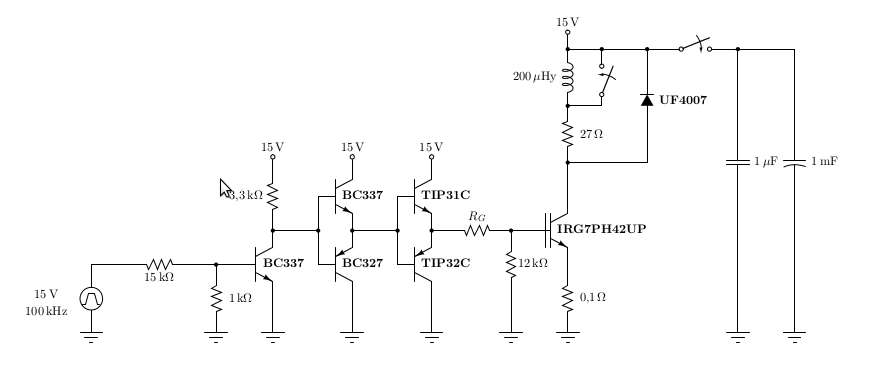
\includegraphics[scale=0.5]{./imagenes/Circuito_IGBT.png}
\caption{Circuito simplificado de disparo de un IGBT.}
 \label{fig:Circuito_IGBT}
\end{center}
\end{figure}

\begin{enumerate}
	\item[•] Explicar por qué los transistores ocupan el lugar que ocupan, es decir, por qué es necesario que cada etapa tenga la capacidad de manejar cada vez mas corriente.
	\item[•]	 Identificar qué función cumple $R_ {G}$ en el circuito. ¿Que sucede si $R_ {G} = 18\unit{\Omega}$ o $R_ {G} = 1k\unit{\Omega}$? Estime la corriente que puede circular por la misma, y calcule en forma aproximada el tiempo que tarda la tensión de Gate del IGBT en establecerse.
	
	La función que cumple $R_ {G}$ en el circuito es la de descargar mas rápido el capacitor asociado al IGBT mientras mas chico sea mas rápido se descargara el capacitor.
	\begin{equation}
	V_{med} = 7.5 \unit{V}	
	\end{equation}
	
	\begin{equation}
	I_{med} = \frac{V_{med}}{R_G}
	\end{equation}
	
	para $R_{G}=18 \unit{\Omega}$
	\begin{equation}
	I_{med}= 624.06 \unit{\mu A} 
	\end{equation}
	
	para $R_{G}=1 \unit{k \Omega}$	
	\begin{equation}
	I_{med}= 576.92 \unit{\mu A} 
	\end{equation}	
	
	
	\item[•] ¿Que función cumple el diodo UF4007?
	
	El diodo UF4007 cumple la función de proteger al transistor ya que limita la tensión en el transistor durante el paso de saturación a corte, proporcionando a través de los diodos un camino para la circulación de la corriente inductiva de la carga.
	
\end{enumerate}

\subsection{Mediciones del circuito}

\subsubsection{Caida de tensión y corriente en el resistor R$_ {G}$}

\begin{figure}[H] %[h] para here [b] para bottom [t] para top [H]+float para aqui si o si
\begin{center}
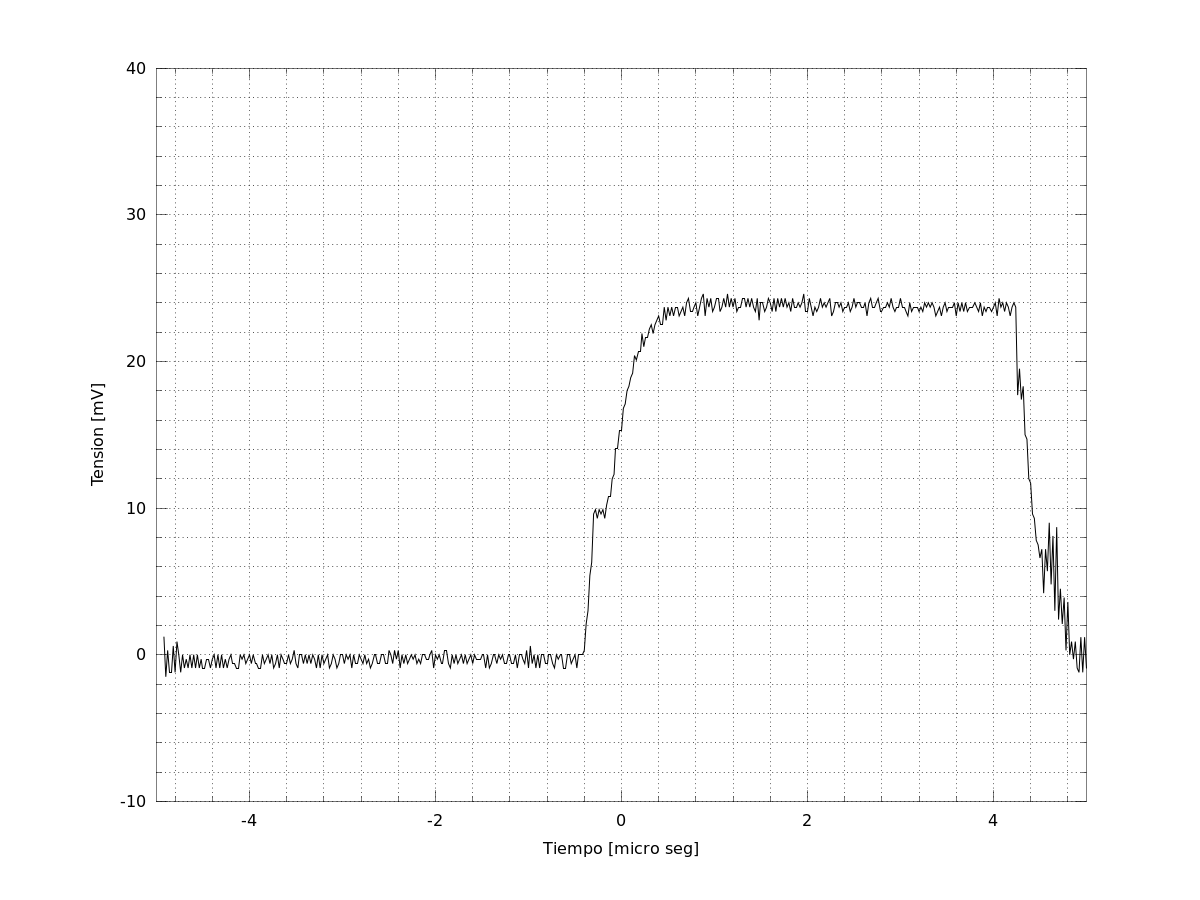
\includegraphics[scale=0.2]{./imagenes/Vrg1.png}
\caption{Caida de tension $V_ {G}$ para $R_ {G}=18\unit{\Omega}$}
 \label{fig:Corriente_IGBT_18ohm}
\end{center}
\end{figure}

\begin{equation}
I_{med} = \frac{1}{T}\sum_{n=0}^N \frac{V_n}{R_g} \Delta t
\end{equation}

\begin{equation}
	I_{med} = 592.13 \unit{\mu A}
\end{equation}

\begin{figure}[H] %[h] para here [b] para bottom [t] para top [H]+float para aqui si o si
\begin{center}
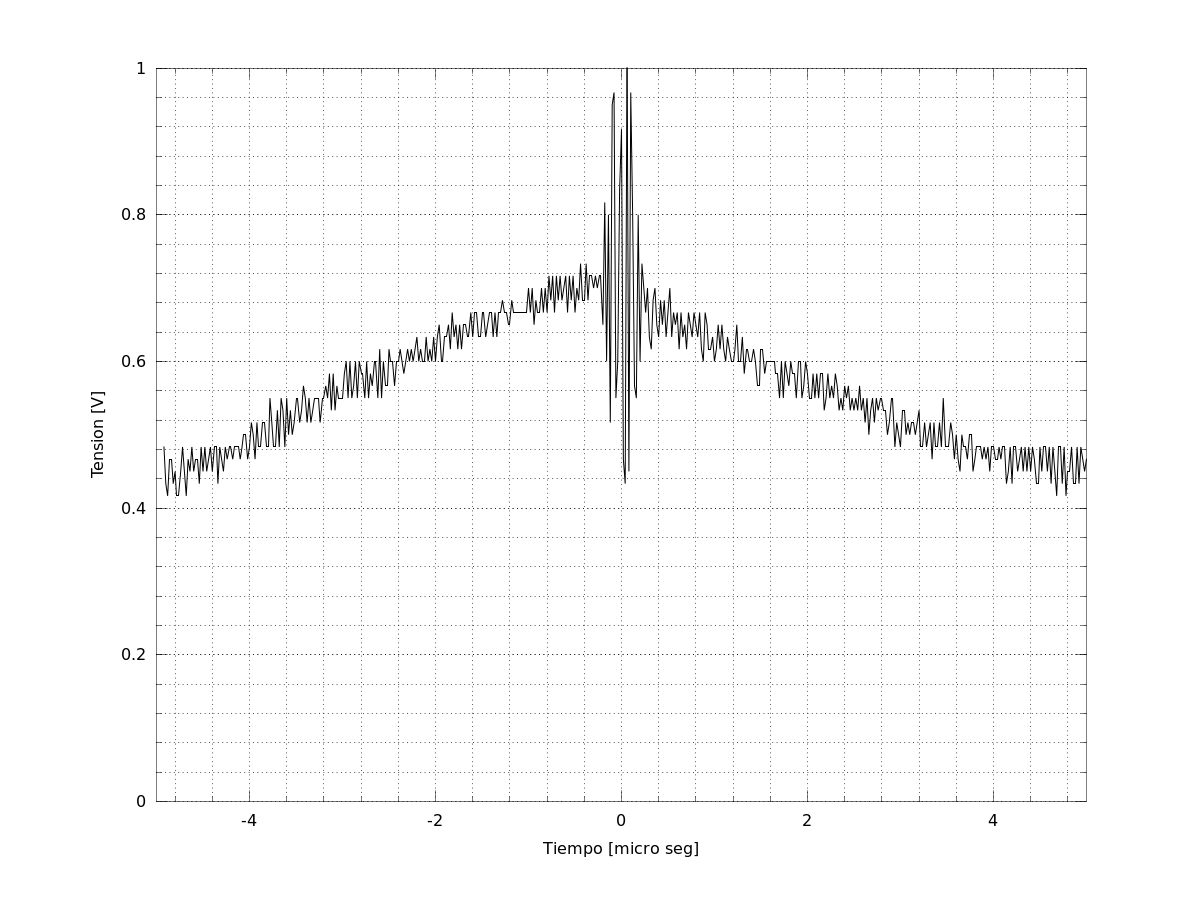
\includegraphics[scale=0.2]{./imagenes/Vrg2.png}
\caption{Caida de tension $V_ {G}$ para $R_ {G}=1\unit{k \Omega}$}
 \label{fig:Corriente_IGBT_1kohm}
\end{center}
\end{figure}

\begin{equation}
	I_{med} = 574.9 \mu A
\end{equation}

\begin{figure}[H] %[h] para here [b] para bottom [t] para top [H]+float para aqui si o si
\begin{center}
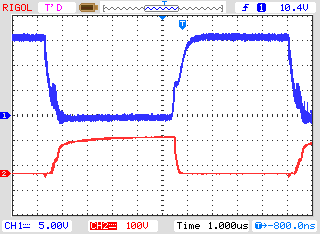
\includegraphics[scale=0.8]{./imagenes/igbt_medicion1_18ohm.png}
\caption{Caida de tension $V_ {G}$ para $R_ {G}=18\unit{\Omega}$}
 \label{fig:Corriente_IGBT_18ohm}
\end{center}
\end{figure}

Se puede observar en la medición que el transistor logra conmutar su estado esto se debe a que R$_ {G}$ es chica por los cual el capacitor asociado al transistor logra descargarse.

\begin{figure}[H] %[h] para here [b] para bottom [t] para top [H]+float para aqui si o si
\begin{center}
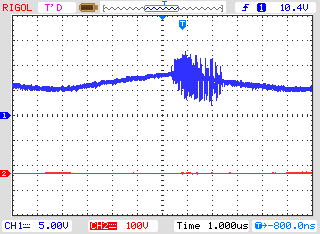
\includegraphics[scale=0.8]{./imagenes/igbt_medicion1_1kohm.png}
\caption{Caida de tension $V_ {G}$ para $R_ {G}=1\unit{k\ Omega}$}
 \label{fig:Corriente_IGBT_1kohm}
\end{center}
\end{figure}

Se puede observar en la medición que el transistor no logra conmutar su estado esto se debe a que $R_{G}$ es grande y no da tiempo a que el  capacitor asociado al transistor logre descargarse. Si la frecuencia de la señal de entrada fuera mas chica el transistor podría llegar a conmutar 

\subsubsection{Capacidad de entrada}

Para calcular el valor de la capacidad de entrada obtuvimos $dV/dt$ mediante cálculos numéricos y obtuvimos la capacidad mediante la siguiente ecuación:

\begin{equation}
C = i\ \frac{dV}{dt}
\end{equation}

y obtuvimos:

\begin{equation}
C = 0,137 \unit{nF}
\end{equation}

Segun la hoja de datos la capacidad de entrada debería ser de $3,338 \unit{nF}$.

\subsubsection{Con el inductor cortocircuitado y los capacitores de salida conectados}

\subsubsection*{Corriente que circula por el IGBT durante las transiciones}

\begin{figure}[H] %[h] para here [b] para bottom [t] para top [H]+float para aqui si o si
\begin{center}
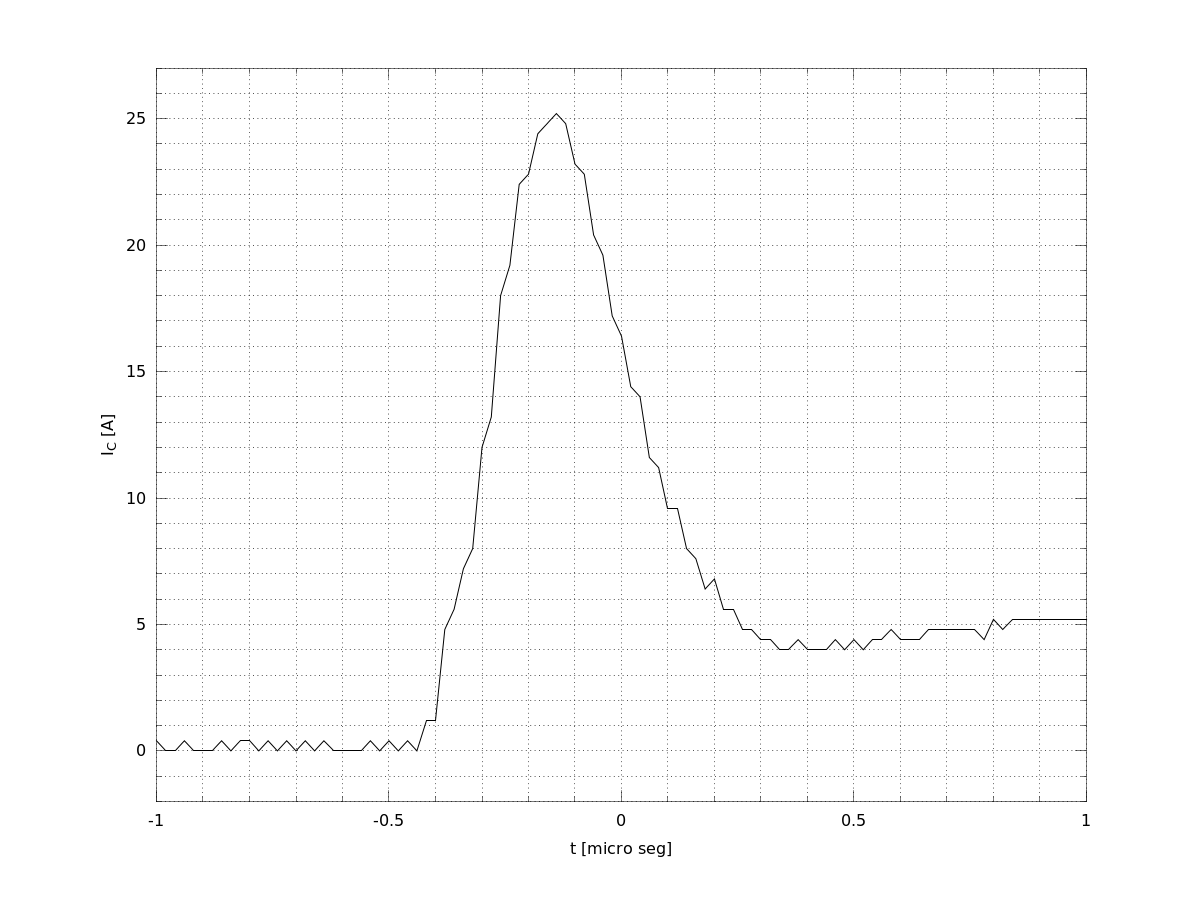
\includegraphics[scale=0.2]{./imagenes/Ic1.png}
\caption{Corriente de colector}
 \label{fig:Ic1}
\end{center}
\end{figure}

\subsubsection*{Energía consumida durante cada transición}

\begin{figure}[H] %[h] para here [b] para bottom [t] para top [H]+float para aqui si o si
\begin{center}
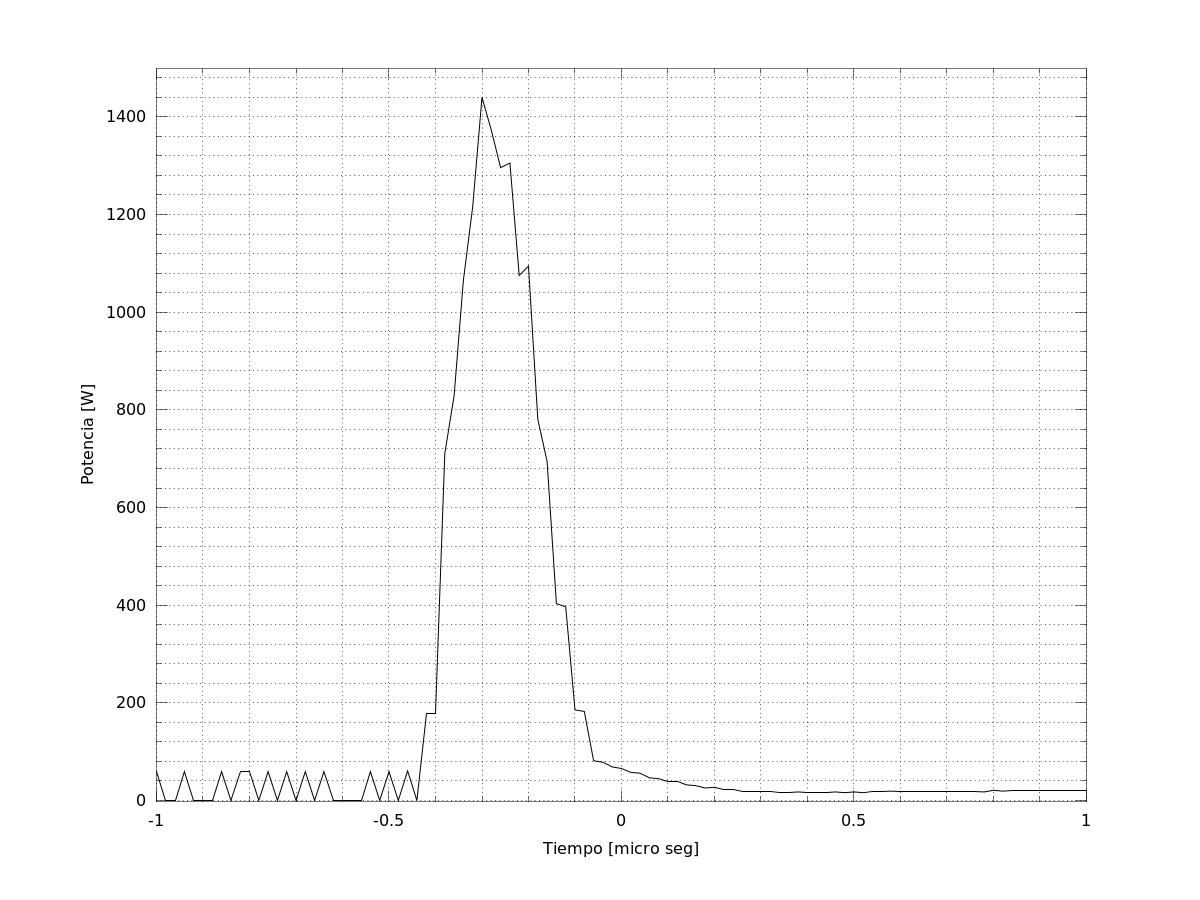
\includegraphics[scale=0.2]{./imagenes/Potencia1.png}
\caption{Potencia instantanea}
 \label{fig:Potencia1}
\end{center}
\end{figure}

En la figura anterior se puede observar la potencia instantánea. La energía disipada en el transistor durante la transición está dada por la integral de la potencia. La integral numérica viene dada por:

\begin{equation}
W = \sum_{n=0}^N P_n \Delta t
\end{equation}

\begin{equation}
	W = 247.32  \unit{\mu J}
\end{equation}
\subsubsection*{Potencia disipada}

La potencia media viene dada por:

\begin{equation}
P_{med} = \frac{1}{T} \int_0^T p(t) dt
\end{equation}

T es el período de conmutación, nosotros estábamos trabajando con $f =
100 \unit{kHz}$.

Pero dado que estamos haciendo cálculos discretos hay que convertir la
integral a una sumatoria quedando:

\begin{equation}
P_{med} = \frac{1}{T} \sum_{n=0}^N p_n \Delta t
\end{equation}

\begin{equation}
	P = 24.732 \unit{W}
\end{equation}

\subsubsection{Con el inductor conectado y los capacitores de salida conectados}

\subsubsection*{Corriente que circula por el IGBT durante las transiciones}

\begin{figure}[H] %[h] para here [b] para bottom [t] para top [H]+float para aqui si o si
\begin{center}
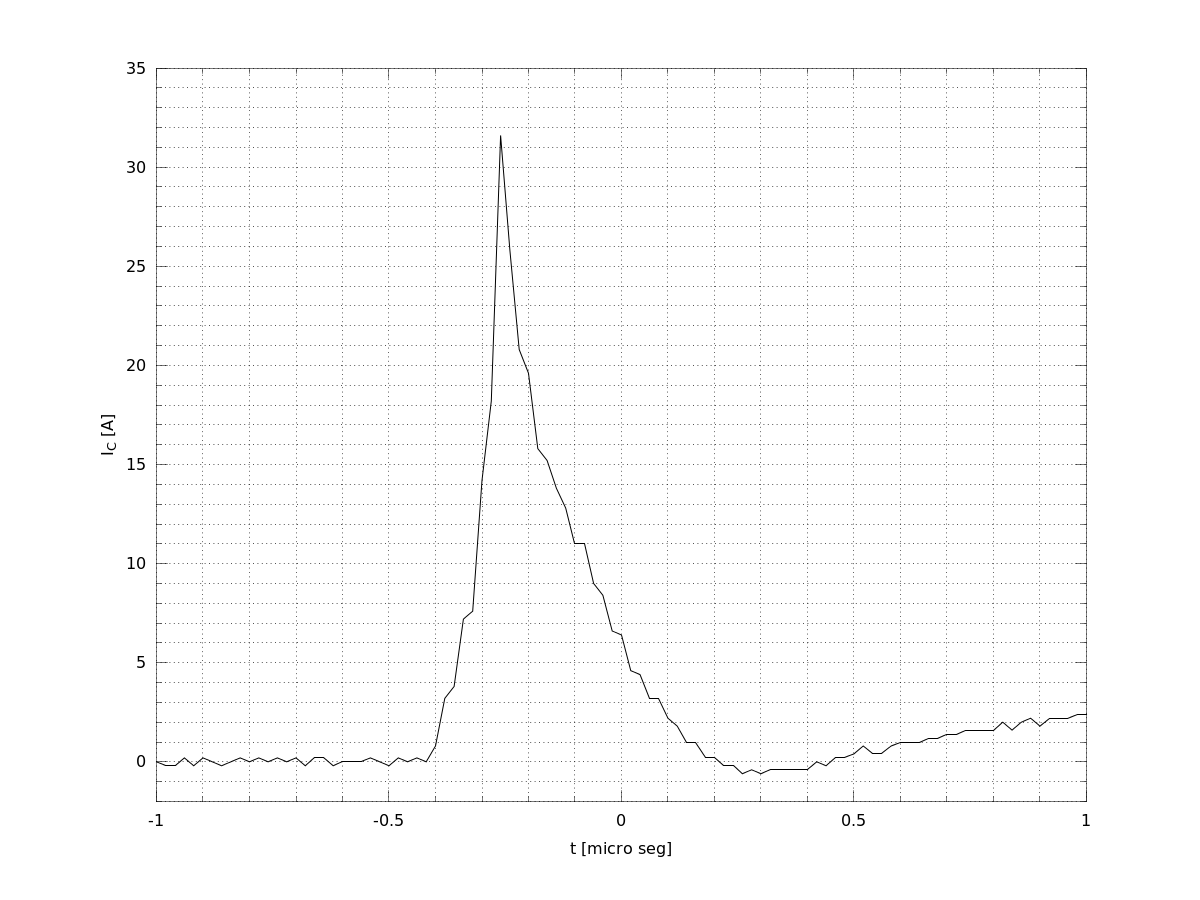
\includegraphics[scale=0.3]{./imagenes/Ic2.png}
\caption{Corriente de colector}
 \label{fig:Ic2}
\end{center}
\end{figure}

\subsubsection*{Energía consumida durante cada transición}

\begin{equation}
W = \sum_{n=0}^N P_n \Delta t
\end{equation}

\begin{equation}
	W = 266.35  \mu J
\end{equation}
\subsubsection*{Potencia disipada}

La potencia media viene dada por:

\begin{equation}
P_{med} = \frac{1}{T} \sum_{n=0}^N p_n \Delta t
\end{equation}

\begin{equation}
	P = 26.635 \unit{W} 
\end{equation}

\subsubsection{Con el inductor conectado y los capacitores de salida desconectados}

\subsubsection*{Corriente que circula por el IGBT durante las transiciones}

\begin{figure}[H] %[h] para here [b] para bottom [t] para top [H]+float para aqui si o si
\begin{center}
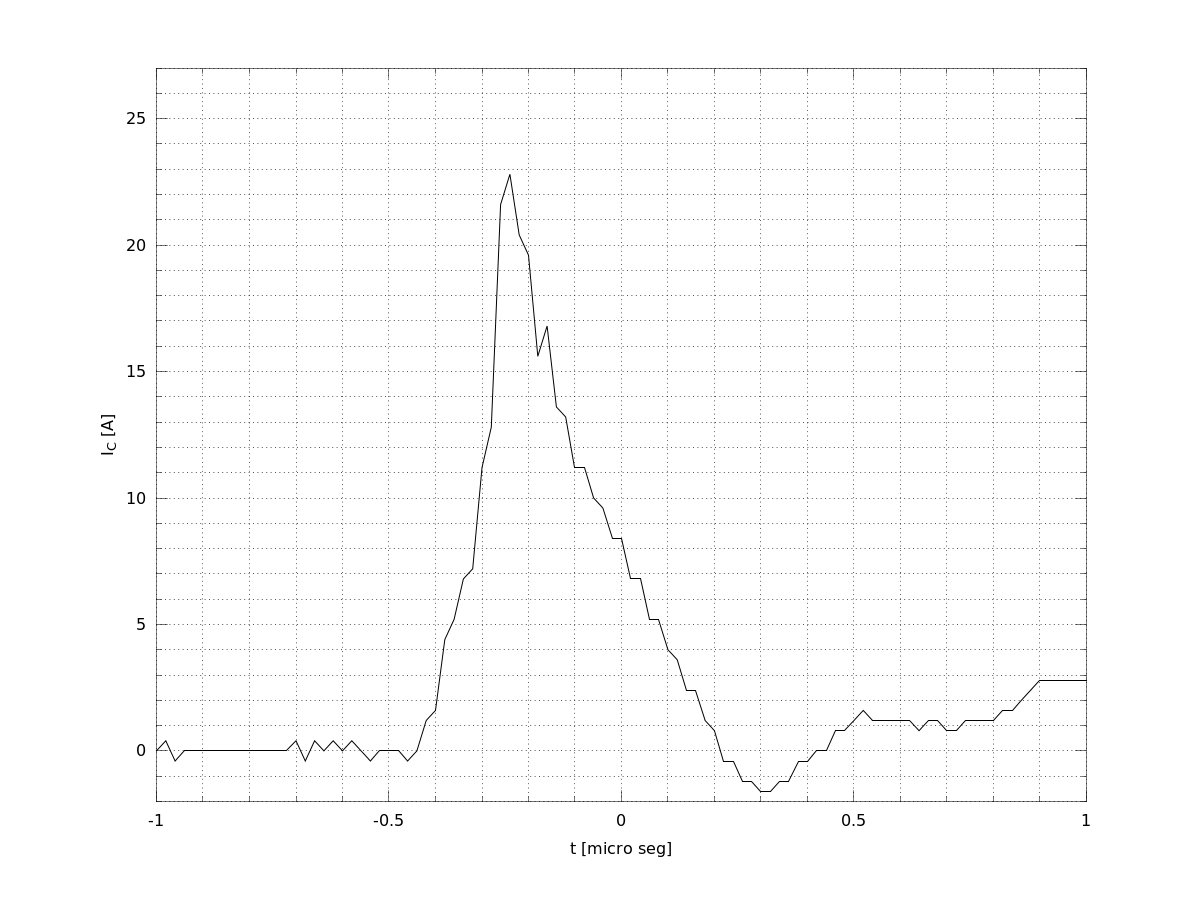
\includegraphics[scale=0.2]{./imagenes/Ic3.png}
\caption{Corriente de colector}
 \label{fig:Ic3}
\end{center}
\end{figure}

\subsubsection*{Energía consumida durante cada transición}

\begin{equation}
W = \sum_{n=0}^N P_n \Delta t
\end{equation}

\begin{equation}
	W = 387.52  \unit{\mu J}
\end{equation}
\subsubsection*{Potencia disipada}

La potencia media viene dada por:

\begin{equation}
P_{med} = \frac{1}{T} \sum_{n=0}^N p_n \Delta t
\end{equation}

\begin{equation}
	P = 38.752 \unit{W} 
\end{equation}

\subsection{Análisis de mediciones}

\begin{enumerate}
	\item[•] ¿Por que es necesario entregar mucha corriente al gate del IGBT?¿Que importancia tiene la resistencia serie del circuito que se encarga de controlar el Gate de este dispositivo?
	
	Es necesario entregar mucha corriente al gate del IGBT ya que se debe superar una tensión para lograr que conmute.
	La resistencia $R_G$ es encargada de descargar el capacitor asociado al IGBT
	
	\item[•]	 ¿Que ocurre si se desea controlar al IGBT con una salida digital típica de un microcontrolador, donde la máxima corriente que se puede entregar es de algunos pocos miliAmperes?
	
	Como la corriente que maneja un microcontrolador es muy chica este no alcanzaría para hacer conmutar el IGBT
	
	\item[•] A partir de la estimación de potencia disipada y de los datos térmicos de las hojas de datos realizar el análisis térmico del IGBT y calcular la temperatura de juntura.
	
	\item[•] ¿Por qué varía la corriente del IGBT con y sin el inductor conectado?
	
\end{enumerate}

\section{Tiristores}

\subsection{Analisis preliminar}

\begin{figure}[H] %[h] para here [b] para bottom [t] para top [H]+float para aqui si o si
\begin{center}
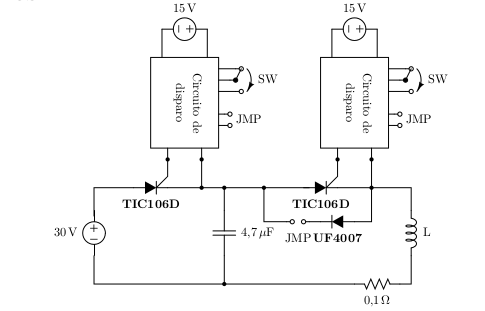
\includegraphics[scale=0.5]{./imagenes/Circuito_Tiristores.png}
\caption{Circuito esquemático simplificado de disparo de dos Tiristores. }
 \label{fig:Circuito_tiristores}
\end{center}
\end{figure}

El circuito es un RLC oscilatorio amortiguado por lo cual se espera ver una tension senoidal amortiguada en la resistencia.
Si el diodo esta conectado la corriente podrá circular por este por lo cual se podrá ver el semiciclo negativo de la senoidal.
Si el diodo no esta conectado solo se podrá ver el semiciclo positivo   

\subsection{Mediciones del circuito}

\subsubsection{Diodo desconectado y disparo corto}

\subsubsection*{Tensión en el inductor y la resistencia respecto del terminal negativo de la fuente}

\begin{figure}[H] %[h] para here [b] para bottom [t] para top [H]+float para aqui si o si
\begin{center}
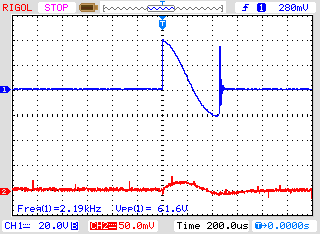
\includegraphics[scale=0.8]{./imagenes/tiristor_medicion1.png}
\caption{Medición de tensión sobre el inductor y la resistencia respecto al terminal negativo de la fuente}
 \label{fig:Med1_tiristor}
\end{center}
\end{figure}

\subsubsection*{Corriente}

\begin{figure}[H] %[h] para here [b] para bottom [t] para top [H]+float para aqui si o si
\begin{center}
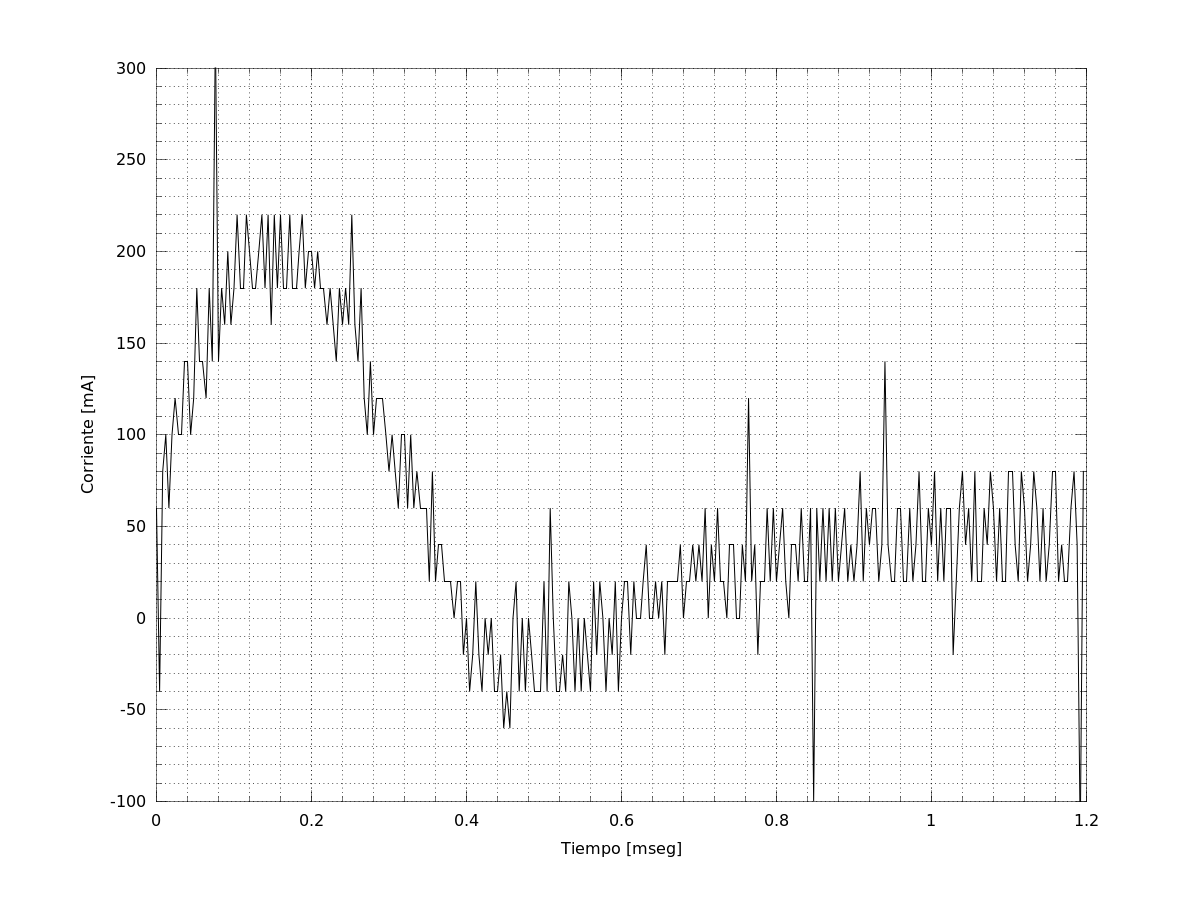
\includegraphics[scale=0.3]{./imagenes/Corriente1.png}
\caption{Corriente que circula por el circuito}
 \label{fig:Corriente1_tiristor}
\end{center}
\end{figure}

\subsubsection{Diodo conectado y disparo corto}

\subsubsection*{Tensión en el inductor y la resistencia respecto del terminal negativo de la fuente}

\begin{figure}[H] %[h] para here [b] para bottom [t] para top [H]+float para aqui si o si
\begin{center}
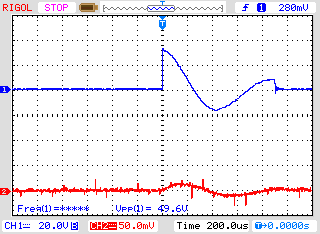
\includegraphics[scale=0.8]{./imagenes/tiristor_medicion2.png}
\caption{Medición de tensión sobre el inductor y la resistencia respecto al terminal negativo de la fuente}
 \label{fig:Med2_tiristor}
\end{center}
\end{figure}

\subsubsection*{Corriente}

\begin{figure}[H] %[h] para here [b] para bottom [t] para top [H]+float para aqui si o si
\begin{center}
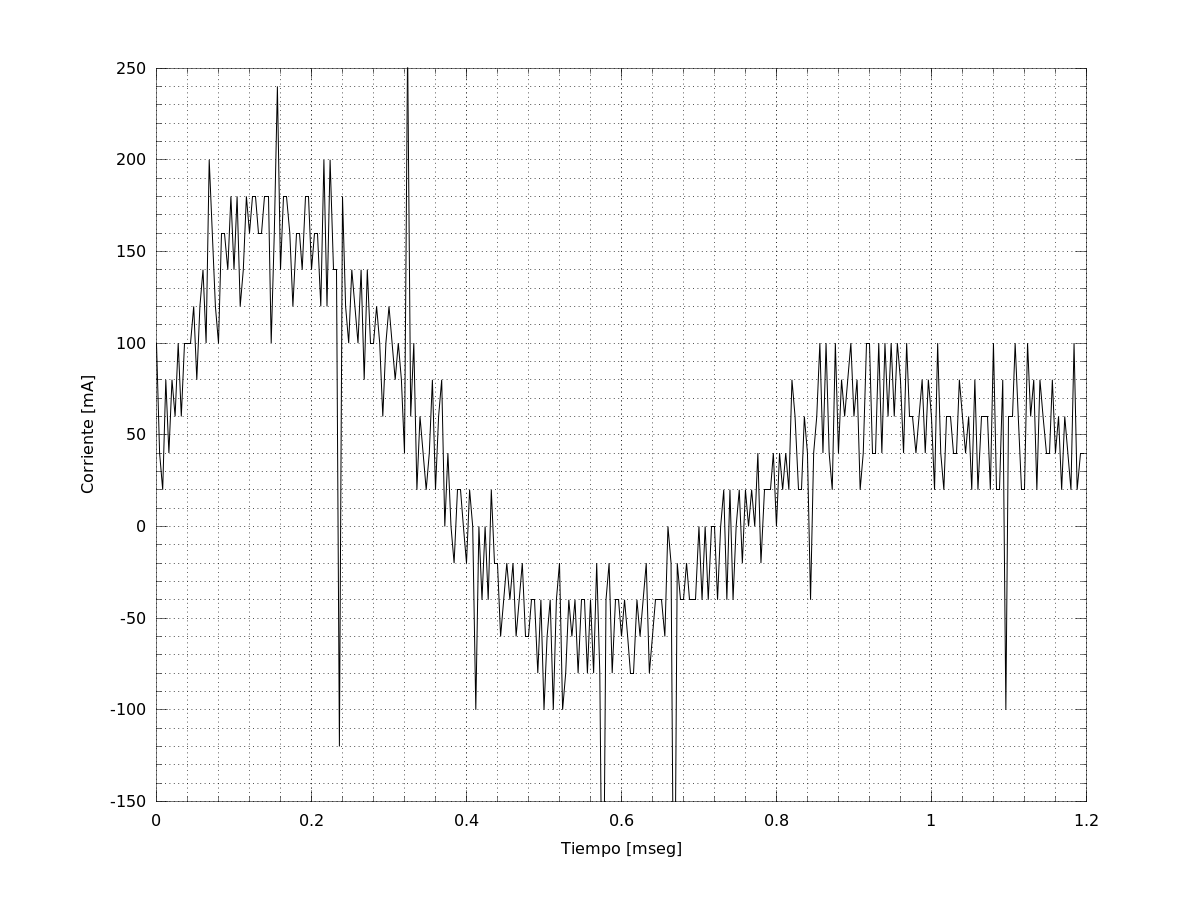
\includegraphics[scale=0.3]{./imagenes/Corriente2.png}
\caption{Corriente que circula por el circuito}
 \label{fig:Corriente2_tiristor}
\end{center}
\end{figure}

\subsubsection{Diodo conectado y disparo largo}

\subsubsection*{Tensión en el inductor y la resistencia respecto del terminal negativo de la fuente}

\begin{figure}[H] %[h] para here [b] para bottom [t] para top [H]+float para aqui si o si
\begin{center}
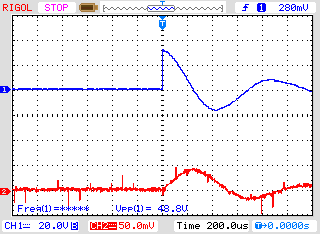
\includegraphics[scale=0.8]{./imagenes/tiristor_medicion3.png}
\caption{Medición de tensión sobre el inductor y la resistencia respecto al terminal negativo de la fuente}
 \label{fig:Med3_tiristor}
\end{center}
\end{figure}

\subsubsection*{Corriente}

\begin{figure}[H] %[h] para here [b] para bottom [t] para top [H]+float para aqui si o si
\begin{center}
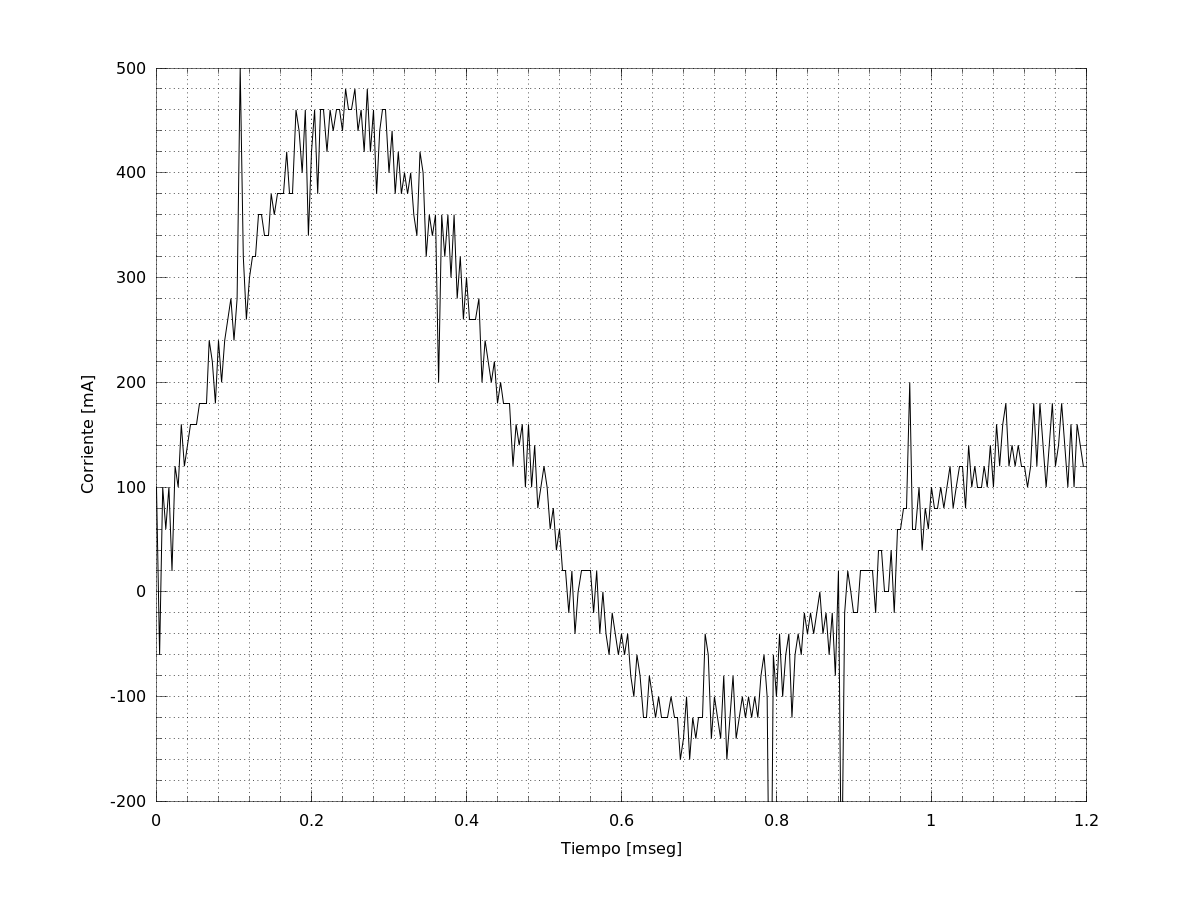
\includegraphics[scale=0.3]{./imagenes/Corriente3.png}
\caption{Corriente que circula por el circuito}
 \label{fig:Corriente3_tiristor}
\end{center}
\end{figure}

\section{Análisis de las mediciones}

\begin{itemize}
	\item ¿Por qué se producen distintas formas de onda para cada una de las configuraciones medidas?
	
Se obtienen resultados distintos ya que estamos realizando cambios en el circuito.
	
	
	\item	 ¿Por qué para cargar el capacitor de $4,7\unit{\mu F}$ alcanza para realizar un disparo corto?
	
El circuito solo esta conformado por la fuente, el tiristor y el capacitor, y solo circula corriente hasta que el tiristor se apague. Esto solo pasa cuando el capacitor está cargado.

\end{itemize}

\section{Conclusión}
Al utilizar dispositivos de potencia es necesario conocer el objetivo del dispositivo de manera de elegir los dispositivos más acordes. Se deben tener en cuenta los mecanismo de protección y bajo que circunstancias se alcanzan resultados óptimos. Por ejemplo al momento de simular un circuito se utiliza una carga inductiva en lugar de una resistiva.
\end{document}